\documentclass[12pt]{article}
\usepackage[margin=2.5cm]{geometry}
\usepackage{enumerate}
\usepackage{amsfonts}
\usepackage{amsmath}
\usepackage{fancyhdr}
\usepackage{amsmath}
\usepackage{amssymb}
\usepackage{amsthm}
\usepackage{mdframed}
\usepackage{graphicx}
\usepackage{subcaption}
\usepackage{adjustbox}
\usepackage{listings}
\usepackage{xcolor}
\usepackage{soul}
\usepackage{booktabs}
\usepackage[utf]{kotex}
\usepackage{hyperref}

\definecolor{codegreen}{rgb}{0,0.6,0}
\definecolor{codegray}{rgb}{0.5,0.5,0.5}
\definecolor{codepurple}{rgb}{0.58,0,0.82}
\definecolor{backcolour}{rgb}{0.95,0.95,0.92}

\lstdefinestyle{mystyle}{
    backgroundcolor=\color{backcolour},
    commentstyle=\color{codegreen},
    keywordstyle=\color{magenta},
    numberstyle=\tiny\color{codegray},
    stringstyle=\color{codepurple},
    basicstyle=\ttfamily\footnotesize,
    breakatwhitespace=false,
    breaklines=true,
    captionpos=b,
    keepspaces=true,
    numbers=left,
    numbersep=5pt,
    showspaces=false,
    showstringspaces=false,
    showtabs=false,
    tabsize=1
}

\lstset{style=mystyle}

\pagestyle{fancy}
\renewcommand{\headrulewidth}{0.4pt}
\lhead{CSC 373}
\rhead{Worksheet 7 Solution}

\begin{document}
\title{CSC373 Worksheet 7 Solution}
\maketitle

\bigskip

\begin{enumerate}[1.]
    \item

    \bigskip

    \begin{mdframed}
    \underline{\textbf{My Work}}

    \bigskip

    The longest simple cycle problem is the problem of finding a cycle of maximum
    length in a graph $^{[5]}$.
    \end{mdframed}

    \bigskip

    The decision problem is, given $k$, to determine whether or not the instance graph
    has a simple cycle of length at least $k$. If yes, output 1. Otherwise, output 0.

    \bigskip

    \begin{mdframed}
    \underline{\textbf{My Work}}

    \bigskip

    The language corresponding to the decision problem is as follows:

    \begin{align*}
        \begin{split}
            \text{LONGEST-SIMPLE-CYCLE} = \{\langle G,v_0,v_1,...,v_k,k\rangle: &\text{$G = (V,E)$ is an undirected graph}\\
            &\text{$k \geq 3$ is an integer,}\\
            &\text{$v_0,v_1,...,v_k \in V$ are distinct,}\\
            &\text{$v_0 = v_k$,}\\
            &\text{There should exist a simple cycle in G}\\
            &\text{with at least $k$ edges}\}
        \end{split}
    \end{align*}
    \end{mdframed}

    \bigskip

    \begin{mdframed}
    \underline{\textbf{Correct Solution:}}

    \bigskip

    The \color{red}problem LONGEST-SIMPLE-CYCLE is a relation that
    associates each instacne of a graph with the longest simple cycle in that graph \color{black}\color{black}.

    \bigskip

    The decision problem is, given $k$, to determine whether or not the instance graph
    has a simple cycle of length at least $k$. If yes, output 1. Otherwise, output 0.

    \bigskip

    The language corresponding to the decision problem is as follows:

    \begin{align*}
        \begin{split}
            \text{LONGEST-SIMPLE-CYCLE} = \{\color{red}\langle G,k\rangle\color{black}: &\text{$G = (V,E)$ is an undirected graph}\\
            &\text{$k \geq \color{red}0\color{black}$ is an integer,}\\
            &\text{There should exist a simple cycle in G}\\
            &\text{with at least $k$ edges}\}
        \end{split}
    \end{align*}
    \end{mdframed}


    % \bigskip

    % \underline{\textbf{Rough Works:}}

    % \bigskip

    % \begin{mdframed}
    % \underline{\textbf{My Work}}

    % \bigskip

    % The longest simple cycle problem is the problem of finding a cycle of maximum
    % length in a graph $^{[5]}$.
    % \end{mdframed}

    % \bigskip

    % The decision problem is, given $k$, to determine whether or not the instance graph
    % has a simple cycle of length at least $k$ edges. If yes, output 1. Otherwise, output 0.

    % \bigskip

    % \begin{mdframed}
    % \underline{\textbf{My Work}}

    % \bigskip

    % The language corresponding to the decision problem is as follows:

    % \begin{align*}
    %     \begin{split}
    %         \text{LONGEST-SIMPLE-CYCLE} = \{\langle G,v_0,v_1,...,v_k,k\rangle: &\text{$G = (V,E)$ is an undirected graph}\\
    %         &\text{$k \geq 3$ is an integer,}\\
    %         &\text{$v_0,v_1,...,v_k \in V$ are distinct,}\\
    %         &\text{$v_0 = v_k$,}\\
    %         &\text{There should exist a simple cycle in G}\\
    %         &\text{with at least $k$ edges}\}
    %     \end{split}
    % \end{align*}
    % \end{mdframed}

    \underline{\textbf{Notes}}

    \begin{itemize}
        \item \textbf{A Cycle in an Undirected Graph}

        \begin{itemize}
            \item A path $\langle v_0,v_1,...,v_k$ forms a cycle if $k \geq 3$, and $v_0 = v_k$.
        \end{itemize}

        \item \textbf{Simple Cycle}

        \begin{itemize}
            \item A cycle is simple if $v_1, v2, ..., v_k$ are distinct
        \end{itemize}
        \item \textbf{Decision Problem}

        \begin{itemize}
            \item Is the problem with yes/no solution
        \end{itemize}

        \bigskip

        \item \textbf{Alphabet}

        \begin{itemize}
            \item Is a finite set of symbols
            \item Is denoted $\Sigma$

            \bigskip

            \underline{\textbf{Example:}}

            \bigskip

            For decision problem, its alphabet is: $\Sigma = \{0,1\}$

            \begin{itemize}
                \item 1 means `yes'
                \item 0 means `no'
            \end{itemize}
        \end{itemize}

        \item \textbf{Language}

        \begin{itemize}
            \item Is any set of strings made of symbols from $\Sigma$
            \item Is denoted $L$

            \bigskip

            \underline{\textbf{Example:}}

            \bigskip

            $L = \{10,11,101,111,1011,1101,10001\}$

            \bigskip

            \item Is denoted $\Sigma^*$ for language of all strings over $\Sigma$ plus empty string $\epsilon$.

            \bigskip

            \underline{\textbf{Example:}}

            \bigskip

            $\Sigma^* = \{\epsilon, 0,1,00,01,11,000,...\}$

            \bigskip

            \underline{\textbf{Example 2:}}

            \bigskip

            The decision problem PATH has the corresponding language

            \bigskip

            \begin{align*}
                \begin{split}\text{PATH} = \{\langle G,U,v,k \rangle:&  \text{$G = (V,E)$ is an undirected graph,}\\&\text{$u,v \in V$,}\\&\text{$k \geq 0$ is an integer, and}\\&\text{tere exists a path from $u$ to $v$ in $G$}\\&\text{consisting of at most $k$ edges}\}\end{split}
            \end{align*}
        \end{itemize}

        \item \textbf{P}

        \begin{itemize}
            \item Is set of problems that can be solved by a deterministic Turing machine in Polynomial time (i.e. $\mathcal{O}(n^k)$) $^{[2]}$.

            \bigskip

            \underline{\textbf{Example:}}

            \bigskip

            \begin{enumerate}[1)]
                \item Shortest path problems
                \item Calculating the greatest common divisor
                \item Finding maximum bipartite matching
            \end{enumerate}

            \bigskip

            \begin{center}
            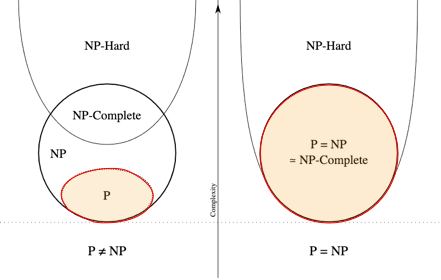
\includegraphics[width=0.7\linewidth]{images/worksheet_7_solution_1.png}
            \end{center}
        \end{itemize}

        \bigskip

        \item \textbf{NP (Non-deterministic Polynominal):}

        \begin{center}
        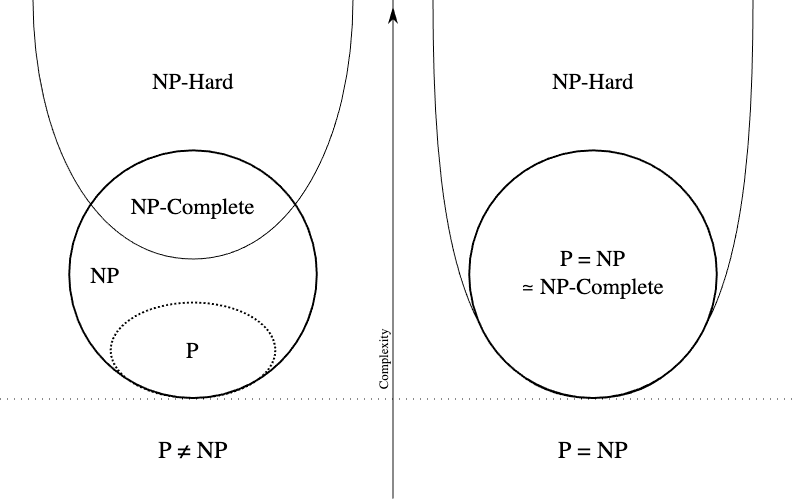
\includegraphics[width=0.7\linewidth]{images/worksheet_7_solution_2.png}
        \end{center}

        \begin{itemize}
            \item Is set of decision problems that can be solved by a Non-deterministic Turing Machine in Polynomial time.$^{[2]}$
            \item Has no particular rule is followed to make a guess $^{[1]}$.
            \item Can be solved in polynominal time via a ``lucky algorithm'', a magical algorithm that always make a right guess $^{[2]}$
            \item $P \subseteq NP$
        \end{itemize}

        \bigskip

        \underline{\textbf{Examples:}}

        \begin{itemize}
            \item Longest-path problems
            \item Hamiltonian Cycle
            \item Graph coloring
        \end{itemize}

        \bigskip

        \item \textbf{NP-Complete Problems:}

        \begin{center}
        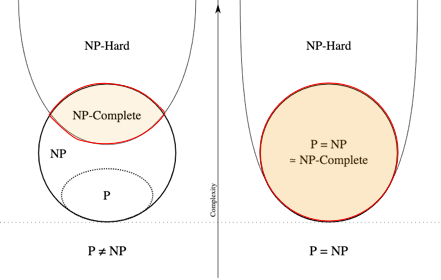
\includegraphics[width=0.7\linewidth]{images/worksheet_7_solution_3.png}
        \end{center}

        \begin{itemize}
            \item A decision problem A is NP-complete (NPC) if

            \begin{enumerate}[1)]
                \item $A \in NP$ and
                \item Every (other) problems $A'$ in NP is reducible to $A$
            \end{enumerate}
            \item Has no efficient solution in polynominal number of steps (not yet) $^{[3]}$
            \item Is not likely that there is an algorithm to make it efficient $^{[3]}$
        \end{itemize}

        \item \textbf{NP-Hard:}

        \bigskip

        \begin{center}
        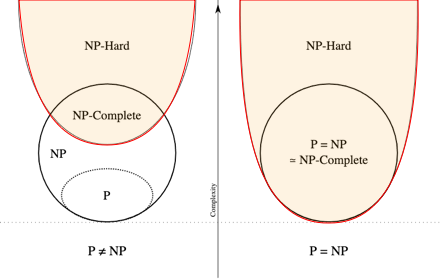
\includegraphics[width=0.7\linewidth]{images/worksheet_7_solution_4.png}
        \end{center}

        \begin{itemize}
            \item A decision problem A is NP-hard if

            \begin{enumerate}[1)]
                \item $A \in NP$ (Not necessarily) and
                \item Every (other) problems $A'$ in NP is reducible to $A$
            \end{enumerate}
            \item NP-Hard means ``at least as hard as any problems in NP''
            \item Does not have to be about decision problems
        \end{itemize}

        \underline{\textbf{Example:}}

        \bigskip

        \begin{enumerate}[1)]
            \item Alan Turing's Halting Problem
        \end{enumerate}

    \end{itemize}

    \bigskip

    \underline{\textbf{References}}

    \bigskip

    \begin{enumerate}[1)]
        \item Encyclopedia Britannica, NP-Complete Problem, \href{https://www.britannica.com/science/NP-complete-problem}{link}
        \item Geeks for Geeks, NP-Completeness, \href{https://www.geeksforgeeks.org/np-completeness-set-1/}{link}
        \item Wikipedia, NP-complete, \href{https://simple.wikipedia.org/wiki/NP-complete}{link}
        \item UCLA UC-Davis, ECS122A Handout on NP-Completeness, \href{https://web.cs.ucdavis.edu/~bai/ECS122A/npcnotes.pdf}{link}
    \end{enumerate}

    \item

    \bigskip

    \underline{\textbf{Notes}}

    \bigskip

    \begin{itemize}
        \item I need help from professors on the meanings behind formalization, and how
        its done :(.

        \begin{itemize}
            \item I am having a lot of difficulty answering this question.
            \item Some of the questions that comes to my mind are
            \begin{enumerate}[1.]
                \item What does it mean when asked to give a formal $x$ of something?
                \item How can I make $x$ formal? What are some thought processes involved in making it formal?
                \item What is the end the first two parts of the problem are looking for?
                \item What does it mean when two are polynominally related?
            \end{enumerate}
        \end{itemize}
        \item \textbf{Encoding}

        \begin{itemize}
            \item Represents problem instances in a way that the program understands
            \item Encoding of a set $S$ is a mapping $e$ from $S$ to the set of binary strings.

            \bigskip

            \underline{\textbf{Example}}

            \bigskip

            Given natural numbers $\mathbb{N} = \{0,1,2,3,4\}$,

            \bigskip

            it's encoding is $\{0,1,10,11,100, ...\}$.

            \bigskip

            Using this encoding, $e(17) = 10001$.

        \end{itemize}
    \end{itemize}

    \item

    \bigskip

    \underline{\textbf{Rough Works:}}

    I need to show whether the algorithm for 0-1 knapsack problem in exercise 16.2-2
    is a polynominal time algorithm.

    \begin{enumerate}[1.]
        \item State that 0-1 knapsack algorithm has running time of $\mathcal{O}(nW)$

        \begin{mdframed}
        Exercise 16.2-2 states that the algorithm has running time of $\mathcal{O}(nW)$
        \end{mdframed}

        \item Check $W$ in $\mathcal{O}(nW)$ is polynominal

        \begin{mdframed}
        The definition of polynominals tells us it is of the form

        \begin{align}
            a_nx^n + a_{n-1}x^{n-1} + ... + a_2x^2 + a_1x + a_0
        \end{align}

        Since we know $W$ represents the total weight of knapsack and is a variable in the form of an integer,
        we can write $W$ is a polynominal.

        \end{mdframed}

        \item Conclude 0-1 knapsack algorithm has polynominal running time

        \begin{mdframed}
        The rule of polynominals tells us product of two polynominals are a polynominal.

        Since we know $n$ is a polynominal and $W$ is a polynominal,
        we can conclude $\mathcal{O}(nW)$ is a polynominal.

        \bigskip

        Thus, we can conclude the 0-1 knapsack problem has a polynominal running time.

        \end{mdframed}

    \end{enumerate}

    \underline{\textbf{Notes}}

    \begin{itemize}
        \item \textbf{Polynominal Time}

        \begin{itemize}
            \item Is expressed in the format $\mathcal{O}(n^k)$.
        \end{itemize}
    \end{itemize}

\end{enumerate}


\end{document}